\section{Session Management}
	Eine Session (Session State Pattern\footnote{\url{http://www.bettersoftwaredesign.org/Design-Patterns/Enterprise-Application-Architecture-Patterns/Session-State-Patterns}}) kann auf dem Client, auf dem Server oder in einer Datenbank abgelegt werden.
	
	\decision{
		\decisionHeader{ARC-SESSION}{Session State}{Architektur}{Architekturdesign}
	}{
		\decisionContent{Client Session State}
		{Auf welchem Tier sollen User Sessions gespeichert werden?}
		{Sowohl das Server- wie das Clientframework beherrschen Session State Management}
		{Diese Entscheidung beeinflusst Client wie Server und bestimmt, ob der der Server zustandsbehaftet oder nicht ausgelegt wird.}
		{"<Server Session State">, "<Database Session State">}
		{"<Client Session State"> ermöglicht die Umsetzung eines zustandslosen Servers. 
			Dadurch wird eine reine Resourcen-basierte Serverschnittstelle möglich.			
		}
		{keine Speziellen}
		{Der Client muss eine Möglichkeit bieten, eine Session zu speichern. Bevorzugt soll dafür ein Session Cookie zum Einsatz kommen.}
		{
			\decisionRef{Server Technologie}{TEC-SERVER},				
			\decisionRef{Client Framework}{TEC-CLIENT-FW}
		}
	}
		
	\section{Datenfluss}			
		Die Übertragung der Daten von und zu den externen Systeme läuft jeweils über den \eeppi-Server, welcher dafür die Rolle eines CORS\footnote{Cross-Origin Resource Sharing: \url{http://de.wikipedia.org/wiki/Cross-Origin_Resource_Sharing}} Proxy einnimmt. 
		Dies ist nötig, da Clients nicht ohne zusätzliche Erlaubnis eines Remoteservers
		auf diesen zugreifen dürfen (Cross Origin Restriction).
		Dies ist ein allgemeines Problem und tritt bei vielen Webanwendungen auf.
		
		Anstatt einen eigenen CORS Proxy zu verwenden, hätte auch ein Drittanbieterservice verwendet werden können.
		Als Beispiels sei hier \hyperlink{http://www.corsproxy.com/}{corsproxy.com} genannt.
		Dies ist ein CORS Proxy in Form eines Webservices.
		Ein CORS Proxy akzeptiert Remote Requests von irgendwelchen Ursprungsadressen und leitet diese dann
		an die entsprechenden Server weiter, die keine Cross-Origin-Requests erlauben.
		
		Wir haben uns entschieden selbst einen kleinen CORS Proxy in unsern Server zu integrieren,
		damit die Daten nicht über fremde Services fliessen und
		\eeppi\ auch in einem lokalen Netzwerk mit beschränktem Internetzugriff betrieben werden kann.
	
	\begin{figure}[H]
		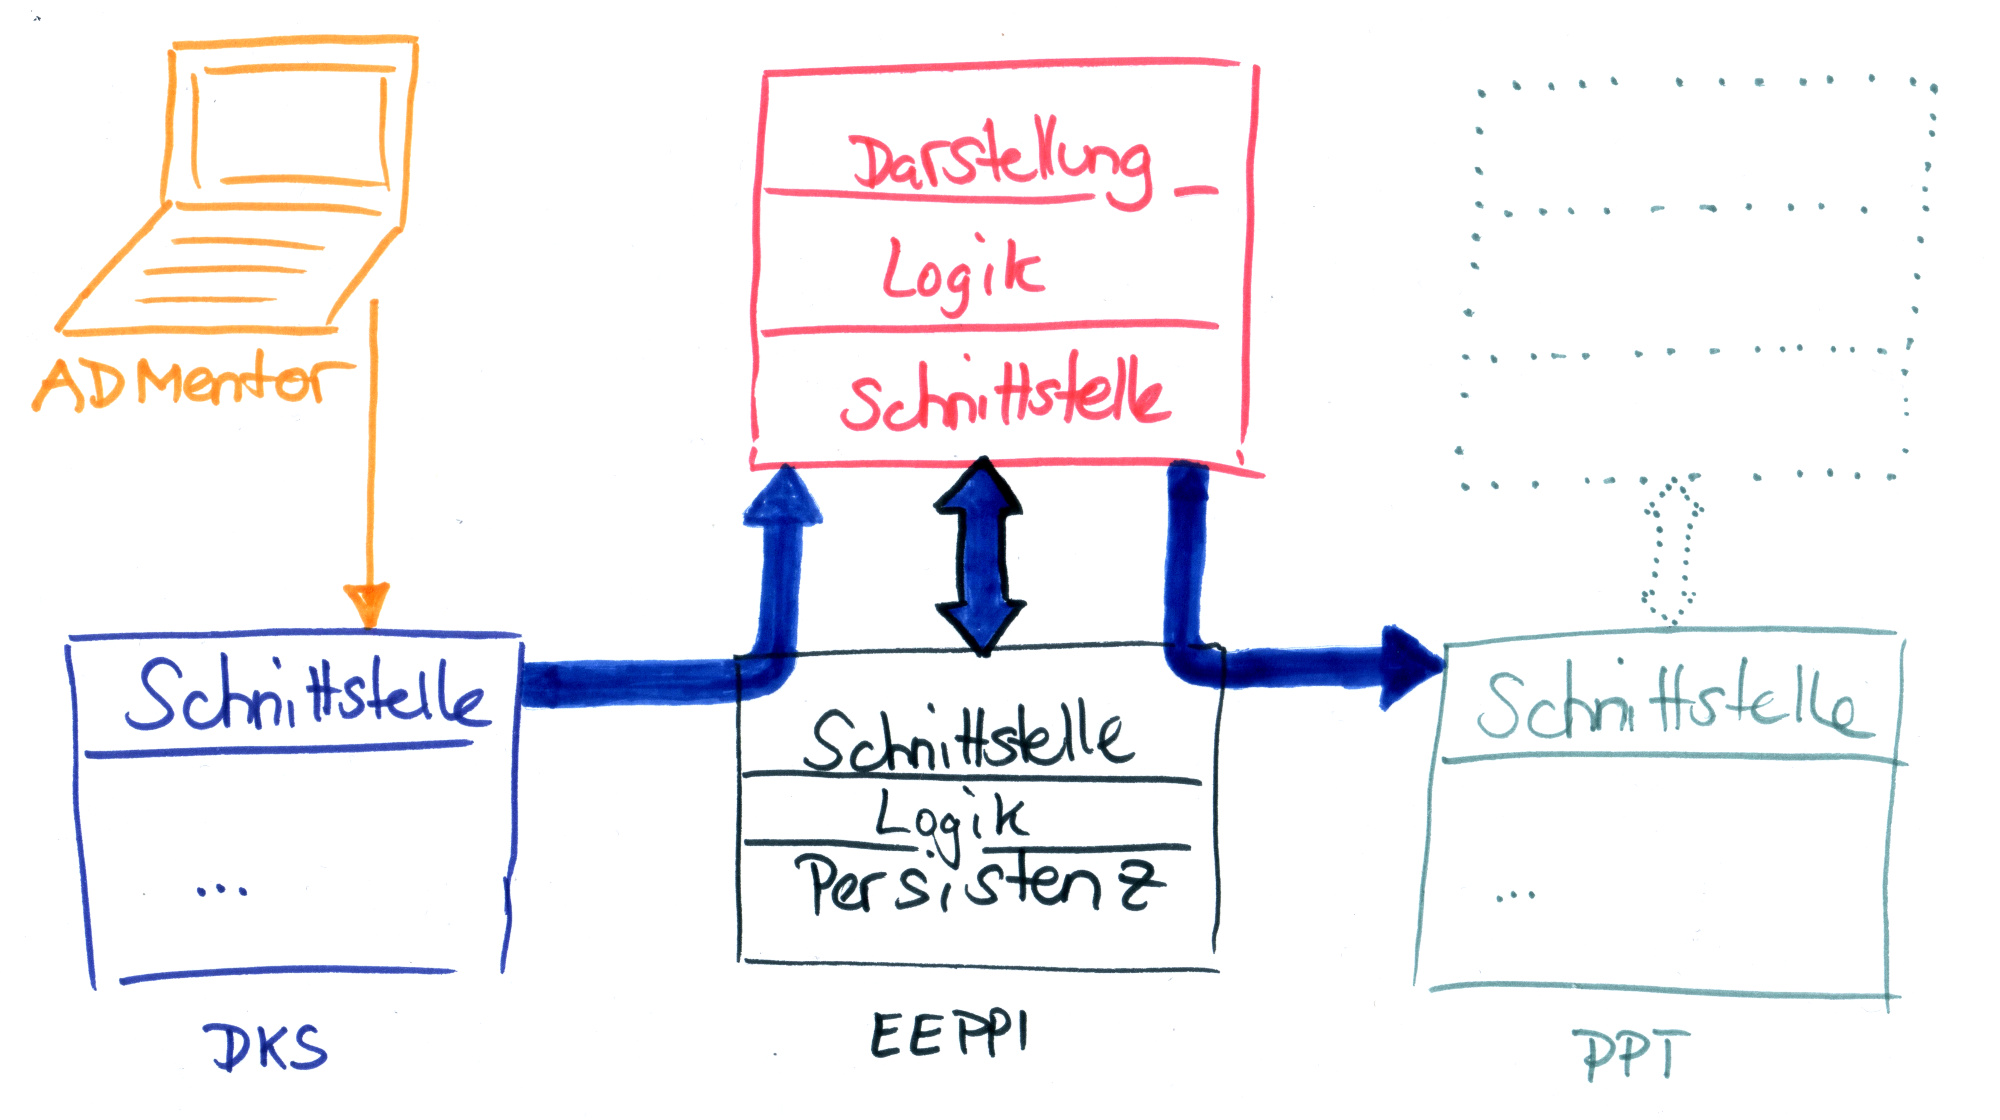
\includegraphics[width=\textwidth]{architecture/media/img/eeppiDataflow.jpg}
		\centering
		\caption{Applikationsdatenfluss mit Beispieldatenquelle ADMentor}
		\label{fig:applicationDataFlow}
	\end{figure}		